%\chapter{Formulation and Raw Materials}
\setlength{\headheight}{12.71342pt}
\addtolength{\topmargin}{-0.71342pt}

\section{Formulation and Raw Materials}
The formulation of the hemp seed bar is an important factor, as it regulates the final nutritional composition and determines the parameters for the upstream and downstream processing steps. Using consistent suppliers and high-quality raw materials are key factors in maintaining a predictable, consistent production. Production as such would decrease faults, which reduces waste and ensures safe a safe high-end product to the final consumer. 

\vspace{1em}
Given the lack of sweetness of hemp seeds, the bar is formulated with naturally sweet components such as dried dates and agave sirup. Along with a caramelly flavor, important cohesiveness of the bar is achieved. The dates are dried which reduces water content and thus increases sugar concentration and intensifies flavor. Minimum processing other than dehydration and pitting ensures valuable components such as micronutrients and fibers are included.

\vspace{1em}
To complement the protein value (which lacks in lysine), potato protein isolate is used. During its production, it undergoes heavy processing which concentrates the protein content while reducing other macronutrients, minerals and vitamins (Wagley et al., 2019).

\vspace{1em}
Rolled oats are used as a structural component. It is chosen as it is a gluten free, cheap, readily available raw material known to consumers. It undergoes dehulling, rolling and steaming, which maintains the high fiber content while inactivating lipase enzymes to prevent oxidation and extend shelf life (Ekelund et al., 2024). Ground flax seeds are also included to account for the loss of dietary fibers in Hemp. The flax seeds are grounded to inhibit toxic effects of cyanogenic glycosides (Nowak et al., 2023).

\vspace{1em}
Preprocessing of hemp seeds aims to partially remove the hull/husk (figure 6). The macronutrient profile of the seed is significantly affected by the processing method. Although the formulation does not involve hemp protein isolate, HPI, many studies on this subject point at the effects of preprocessing. 

\vspace{1em}
For example, a study by House et al., 2010 evaluated HPI derived from whole seeds, hemp seed meal, and solely hulls. The study could show that the amino acid composition is different among the three processed raw materials. In the works by Shen et al., 2020 the HPI of dehulled and whole seeds were comprehensively investigated in terms of aromatic components, colour, and protein characterization. Dehulled seeds would increase the extraction yield by 21.52 \% and protein recovery yield (46.90\%) of the HPI. Naturally, the HPI with whole seeds would contain increased amounts of lipids and carbohydrates. The preprocessing also had a profound impact on colour, were whole seeds generated a darker coloured HPI. This matter is further explained in the section “4.1 Effects on Processing”

\vspace{1em}
Vanilla extract, cocoa and sea salt are used to characterize the aroma of the bar. Potentially masking some of the earthy off-flavours from the other ingredients. 


\begin{figure}[h]
    \centering
    \begin{subfigure}{0.45\textwidth}
        \centering
        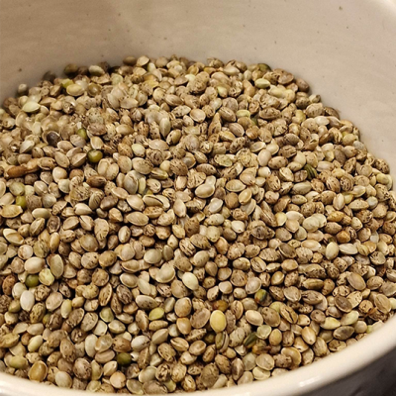
\includegraphics[width=\linewidth]{Figures/fig_formulation_06.png}
        \caption{Whole hemp seeds}
        \label{fig:whole_hemp}
    \end{subfigure}
    \hfill
    \begin{subfigure}{0.45\textwidth}
        \centering
        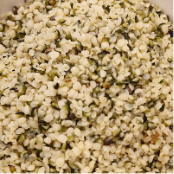
\includegraphics[width=\linewidth]{Figures/fig_formulation_06.1.png}
        \caption{Dehulled hemp seeds}
        \label{fig:dehulled_hemp}
    \end{subfigure}
    \caption{Whole and dehulled hemp seeds (Svensk Hampaindustri, 2025).}
    \label{fig:whole_dehulled}
\end{figure}

